\chapter{Reducing Influence of External Noise}
\section{Generation of Insect-like Signals by External Noise}



\newpage

\section{Efficacy of Physical Noise Reduction}

The developed vibro-acoustic insect detection system provided sufficient physical soundproofing that enabled measurement of insect signatures with high SNR by the integrated piezoelectric sensors without interference from external noise. Strong external noise with impulse characteristics, however, could still penerate inside the enclosure and generate signals similar to those produced by insects and mask their presence.

Although different types of external noise were simulated during recordings through loudspeakers, recordings of solo male speech demonstrated the most significant interference and was selected for the subset. The speech was played at varying sound levels from \SIrange{60}{100}{\deci\bel A} at \SI{10}{\deci\bel} increments and controlled using the calibrated Extech 407730 Digital Sound Level Meter from Teledyne FLIR \cite{Extech407730Digitala}. Spectrograms of the speech signal at \SI{90}{\deci\bel A} measured by the piezoelectric sensors, channels zero and one, the collocated microphones, channels four and five, and the external microphone, channel seven, are presented in Figure \ref{fig: spectrogram insect-like noise}. The scales of the piezoelectric and microphone spectrograms are adjusted and differentiated to highlight the impulses.

\begin{figure}[H]%
	\centering
	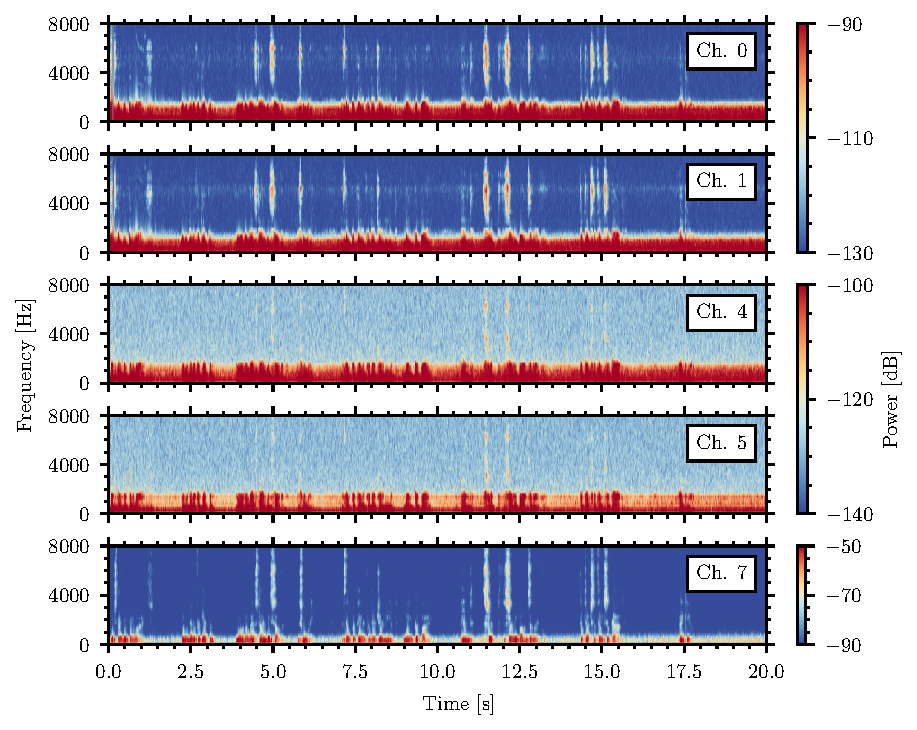
\includegraphics[width=\textwidth]{figures/5_1_insect_like_noise.pdf}%
	\caption{Spectrogram from piezoelectric and acoustic microphones during external noise, amplified speech at \SI{90}{\deci\bel A}. Insect like pulses are visible in all channels}%
	\label{fig: spectrogram insect-like noise}%
\end{figure}

The spectrograms show the variation of the external signal as it propogates through the system. The impulses are similar to the insect signals presented in Figure 5 of the previous publication \cite{kadyrovVibroAcousticSignaturesVarious2024}. The NSPA values calculated from the noise recordings range from \SIrange{39.34}{69.41}{\deci\bel} at noise levels from \SIrange{60}{100}{\deci\bel A}, respectively, which are comparable or exceed those of the insect signals. This demonstrates a challenge in setting a detection threshold, $T$, that can distinguish between insect signals and external noise without incurring false positives or negatives.

% \subsection{Calibration of External Microphone}

% Since the POM-2735P-R microphone is designed to capture sound pressure as a varying electrical signal, beyond specifying a \SI{-35}{\deci\bel} sensitivity, the manufacturer does not provide a calibration curve or built-in circuitry to correct for minor variations. Calibration is required to ensure accurate and consistent measurements. The external microphone is not openly exposed so performing calibration using an acoustic calibrator to IEC 61094 standards was not feasible \cite{auCalibrationMicrophonesAccordance2017}. Instead, recording where the Exotech Sound Pressure Meter was utilized to measure the simulated external noise were used fit the difference in the calculated SPL of the channel seven microphone. An A-weighting filter was applied to the raw signal from channel seven, the root-mean square (RMS) value was computed, and converted to decibels using the standard reference pressure of \SI{20}{\micro\pascal} \cite{chungCalibrationMattersSound2023}. The difference in the SPL measurements between the channel seven microphone and the SPL meter was used to fit a calibration curve using linear regression. Figure \ref{fig:external_microphone_calibration} shows the calibration fit for the channel seven microphone with the SPL measurements.

% \begin{figure}[!htbp]
% 	\centering
% 	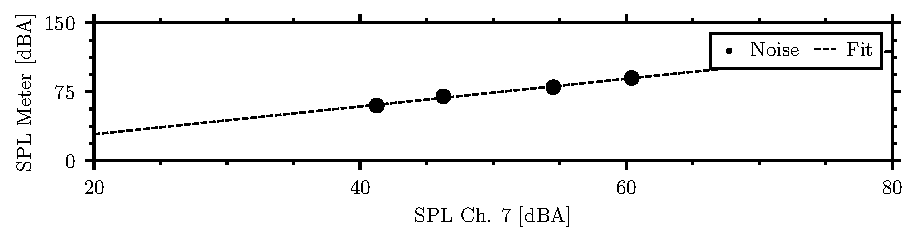
\includegraphics[width=\textwidth]{figures/external_noise/ch7_spl_graph.pdf}
% 	\caption{Calibration of microphone channel 7 with SPL measurements}
% 	\label{fig:external_microphone_calibration}
% \end{figure}

% By applying the calibration curve obtained from the reference sound level meter, the output of the external microphone can be adjusted to estimate the true sound pressure levels of the environment. 

\subsection{Influence of Ambient Noise}

The developed vibro-acoustic insect detection system provided sufficient physical soundproofing that enabled measurement of insect signatures with high SNR by the integrated piezoelectric sensors without interference from external noise. Strong external noise with impulse characteristics, however, could still penerate inside the enclosure and generate signals similar to those produced by insects and mask their presence.

Although different types of external noise were simulated during recordings through loudspeakers, recordings of solo male speech demonstrated the most significant interference and was selected for the subset. The speech was played at varying sound levels from \SIrange{60}{100}{\deci\bel A} at \SI{10}{\deci\bel} increments and controlled using the calibrated Extech 407730 Digital Sound Level Meter from Teledyne FLIR \cite{Extech407730Digitala}. Spectrograms of the speech signal at \SI{90}{\deci\bel A} measured by the piezoelectric sensors, channels zero and one, the collocated microphones, channels four and five, and the external microphone, channel seven, are presented in Figure \ref{fig: spectrogram insect-like noise}. The scales of the piezoelectric and microphone spectrograms are adjusted and differentiated to highlight the impulses.

\begin{figure}[H]%
	\centering
	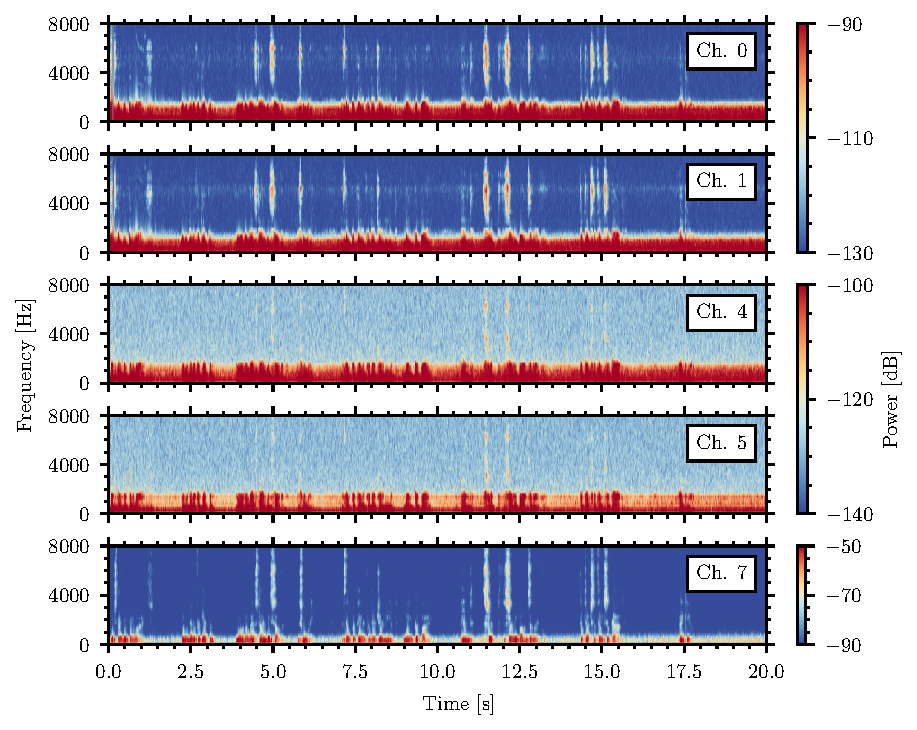
\includegraphics[width=\textwidth]{figures/5_1_insect_like_noise.pdf}%
	\caption{Spectrogram from piezoelectric and acoustic microphones during external noise, amplified speech at \SI{90}{\deci\bel A}. Insect like pulses are visible in all channels}%
	\label{fig: spectrogram insect-like noise}%
\end{figure}

The spectrograms show the variation of the external signal as it propogates through the system. The impulses are similar to the insect signals presented in Figure 5 of the previous publication \cite{kadyrovVibroAcousticSignaturesVarious2024}. The NSPA values calculated from the noise recordings range from \SIrange{39.34}{69.41}{\deci\bel} at noise levels from \SIrange{60}{100}{\deci\bel A}, respectively, which are comparable or exceed those of the insect signals. This demonstrates a challenge in setting a detection threshold, $T$, that can distinguish between insect signals and external noise without incurring false positives or negatives.

\newpage
Figure \ref{fig:waveform_comparison} juxtaposes the filtered, enveloped, and normalized waveforms for the \textit{T. confusum} in flour and the \textit{C. maculatus} in oatmeal with the \SI{60}{\decibel A} and \SI{90}{\deci\bel A} external noise. 

\begin{figure}[!htbp]
	\centering

	\begin{subfigure}{0.45\textwidth}
		\centering
		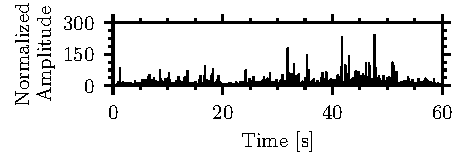
\includegraphics[width=\textwidth]{figures/normalization/Confused flour beetle_Flour_waveform_normalized_small (500-6000).pdf}
		\caption{\textit{T. confusum} in flour}
		\label{fig:cfb_flour_waveform}
	\end{subfigure}
	\hfill
	\begin{subfigure}{0.45\textwidth}
		\centering
		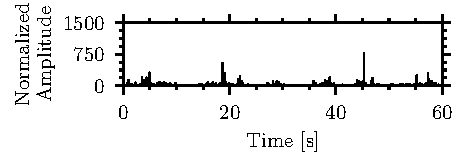
\includegraphics[width=\textwidth]{figures/normalization/Bean beetle_Oatmeal_waveform_normalized_small (500-6000).pdf}
		\caption{\textit{C. maculatus} in oatmeal}
		\label{fig:bb_oatmeal_waveform}
	\end{subfigure}

	\vspace{1em}

	\begin{subfigure}{0.45\textwidth}
		\centering
		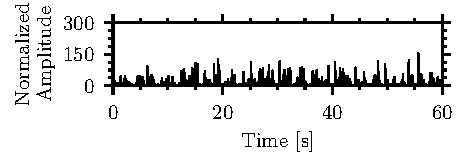
\includegraphics[width=\textwidth]{figures/normalization/Noise_60 dBA_waveform_normalized_small (500-6000).pdf}
		\caption{60 dBA external noise}
		\label{fig:noise_60_waveform}
	\end{subfigure}
	\hfill
	\begin{subfigure}{0.45\textwidth}
		\centering
		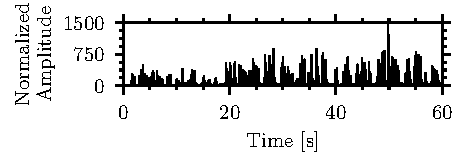
\includegraphics[width=\textwidth]{figures/normalization/Noise_90 dBA_waveform_normalized_small (500-6000).pdf}
		\caption{90 dBA external noise}
		\label{fig:noise_90_waveform}
	\end{subfigure}

	\caption{Processed signals from insects and external noise using the \SIrange{500}{6000}{\hertz} frequency band}
	\label{fig:waveform_comparison}
\end{figure}

Analyzing the spectra of the signals reveals that a more detailed spectral analysis can provide a means to differentiate between insect generated impulses and those from external noise. Figure \ref{fig:spectral_comparison} compares the spectra measured by a piezoelectric sensor channel zero during \SI{90}{\deci\bel A} external noise with \textit{T. confusum} in flour and \textit{C. maculatus} in oatmeal. 

\begin{figure}[!htbp]
	\centering
	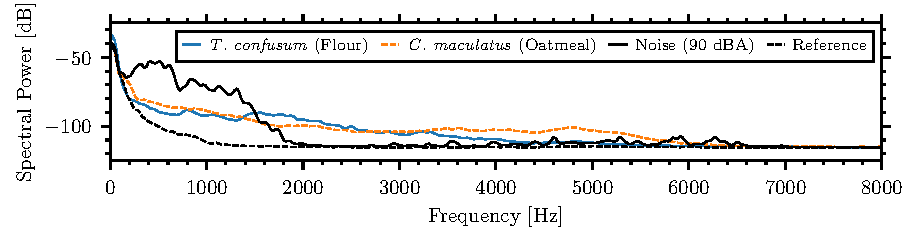
\includegraphics[width=\textwidth]{figures/external_noise/spectra_comparison.pdf}
	\caption{Comparison of insect, noise, and reference spectra}
	\label{fig:spectral_comparison}
\end{figure}

Although the noise signal permeates the internal sensor, especially at frequencies below \SI{1500}{\hertz}, the insect generated impulses have a higher spectral power above that frequency. This demonstrates that this lower frequency bound can be effectively utilized for detection purposes even in the presence of strong ambient noise.

\newpage
\subsection{Optimizing Frequency Range to Limit External Noise Influence}

The NSPA algorithm was parametrized in order to find the lower and upper frequency limits that would enable the optimal detection of insect signals while minimizing the impact of external noise. Twenty samples of the insect signals representative of the median strength for each respective insect-material pairing combination were selected for analysis. The frequency bands were systematically varied and the respective NSPA values calculated and compared to the NSPA values of the external noise at \SI{90}{\deci\bel A} at the same range. 

% Figure \ref{fig:nspa_diff_grid} illustrates the magnitude of the difference between the insect and noise NSPA values at different low, $\omega_1$, and high, $\omega_2$, frequency combinations. 

% \begin{figure}[!htbp]
% 	\centering
% 	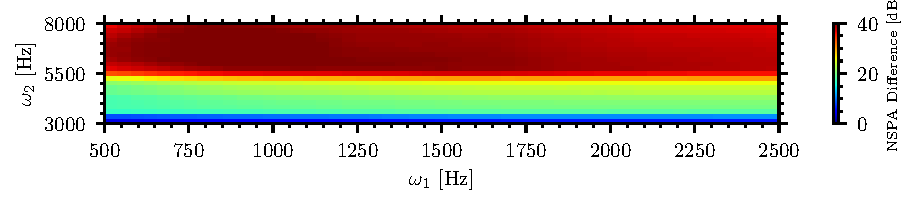
\includegraphics[width=\textwidth]{figures/nspa_optimization/nspa_diff_grid.pdf}
% 	\caption{NSPA difference between insect and noise signals at different filter frequency range combinations}
% 	\label{fig:nspa_diff_grid}
% \end{figure}

Although the NSPA difference significantly increases when the low range is above \SI{1500}{\hertz}, the high frequency bound plays a less critical role maximizing at around \SI{4000}{\hertz}. Focusing on the low frequency range, Figure \ref{fig:nspa_low_frequency} shows the NSPA difference between the insect and noise signals as the low frequency bound is varied while the high frequency bound is fixed at \SI{6000}{\hertz}. The optimal low frequency bound was determined to be \SI{1565}{\hertz} which was where the maximal NSPA difference converged to within \SI{5}{\percent}.  

\begin{figure}[!htbp]
	\centering
	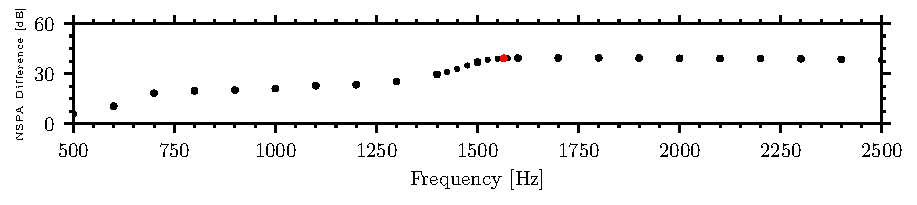
\includegraphics[width=\textwidth]{figures/nspa_optimization/nspa_low_frequency.pdf}
	\caption{Comparison of insect, noise, and reference spectra}
	\label{fig:nspa_low_frequency}
\end{figure}

% Table \ref{tab:optimal_frequency} compares the averaged NSPA values of the twenty insect-material samples and noise from \SIrange{60}{90}{\deci\bel A} using the original \SIrange{500}{6000}{\hertz} and the \SIrange{1565}{6000}{\hertz} frequency bands. 

% \begin{table}[htbp!]
% 	\centering
% 	\caption{Comparison of insect and noise NSPA values at different frequency bands \label{tab:optimal_frequency}}
% 	\begin{tabular}{lrr}
% 		\toprule
% 		\textbf{Subject}     & \textbf{\SIrange{500}{6000}{\hertz}} & \textbf{\SIrange{1565}{6000}{\hertz}} \\
% 		\midrule
% 		Insect (Averaged) & 47.43 & 47.39 \\
% 		Noise (\SI{61}{\deci\bel A}) & 39.31 & 8.39 \\
% 		Noise (\SI{68.46}{\deci\bel A}) & 45.39 & 10.26 \\
% 		Noise (\SI{80.95}{\deci\bel A}) & 54.81 & 17.91 \\
% 		Noise (\SI{89.88}{\deci\bel A}) & 58.19 & 26.21 \\
% 		\bottomrule
% 	\end{tabular}
% \end{table}

% The NSPA values of the insects remain nearly unchanged while the NSPA values of the noise are significantly reduced. 

Figure \ref{fig:waveform_comparison_optimized} compares the normalized waveforms of the insect signals and external noise using the optimized frequency band and demonstrate that the insect impulses remain distinct while the noise impulses are significantly diminished.

\begin{figure}[!htbp]
	\centering

	\begin{subfigure}{0.45\textwidth}
		\centering
		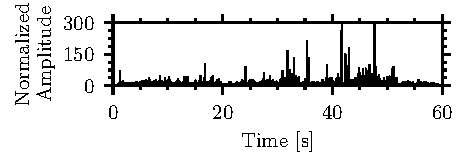
\includegraphics[width=\textwidth]{figures/normalization/Confused flour beetle_Flour_waveform_normalized_small (1565-6000).pdf}
		\caption{\textit{T. confusum} in flour}
		\label{fig:cfb_flour_waveform_optimal_freq}
	\end{subfigure}
	\hfill
	\begin{subfigure}{0.45\textwidth}
		\centering
		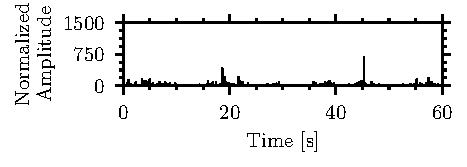
\includegraphics[width=\textwidth]{figures/normalization/Bean beetle_Oatmeal_waveform_normalized_small (1565-6000).pdf}
		\caption{\textit{C. maculatus} in oatmeal}
		\label{fig:bb_oatmeal_waveform_optimal_freq}
	\end{subfigure}

	\vspace{1em}

	\begin{subfigure}{0.45\textwidth}
		\centering
		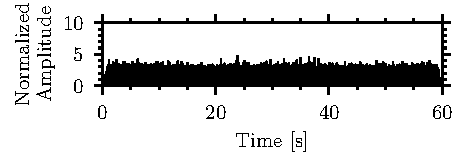
\includegraphics[width=\textwidth]{figures/normalization/Noise_60 dBA_waveform_normalized_small (1565-6000).pdf}
		\caption{60 dBA external noise}
		\label{fig:noise_60_waveform_optimal_freq}
	\end{subfigure}
	\hfill
	\begin{subfigure}{0.45\textwidth}
		\centering
		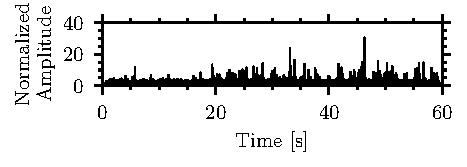
\includegraphics[width=\textwidth]{figures/normalization/Noise_90 dBA_waveform_normalized_small (1565-6000).pdf}
		\caption{90 dBA external noise}
		\label{fig:noise_90_waveform_optimal_freq}
	\end{subfigure}

	\caption{Comparison of normalized waveforms: insects vs external noise}
	\label{fig:waveform_comparison_optimized}
\end{figure}


% Even at \SI{60}{\deci\bel A} external noise, the piezoelectric discs have a significant response especially from \SIrange{200}{1400}{\hertz} where the SNR is almost identical to the external microphone channel seven. This not only indicates that the piezoelectric discs pick up external noise, even through the physical insulation, but also compromises using the \SIrange{500}{6000}{\hertz} frequency range for detection. Figure \ref{fig:spectrogram_41} shows the spectrograms from the internal piezoelectric channels and the external microphone channel seven during the \SI{60}{\deci\bel} noise.

% \begin{figure}[!htbp]
% 	\centering
% 	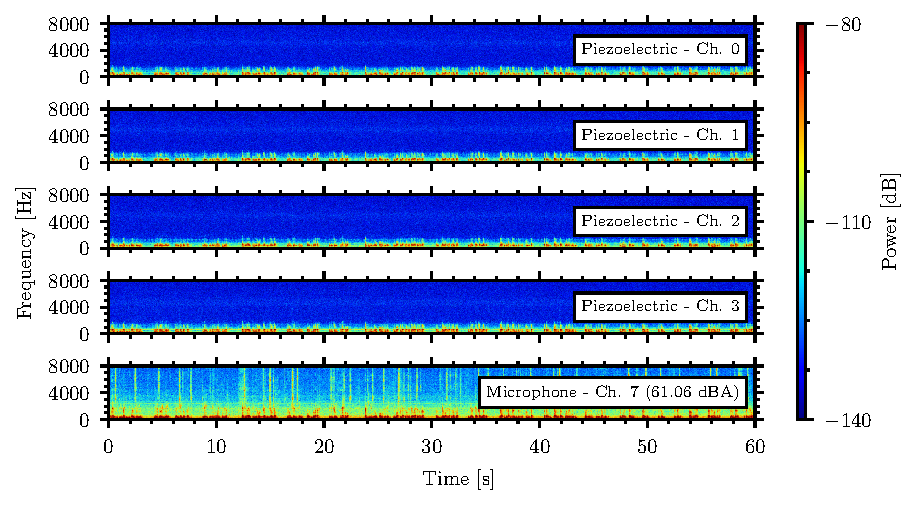
\includegraphics[width=\textwidth]{figures/external_noise/spectrogram_41.pdf}
% 	\caption{Spectrogram display of \SI{60}{\deci\bel A} external noise}
% 	\label{fig:spectrogram_41}
% \end{figure}

% \newpage
% The spectrograms show the infiltration of the impulses from the noise, distinct in channel seven, manifest synchronously in the piezoelectric channels. This is also clearly seen in Figure \ref{fig:waveform_41} which shows the filtered, enveloped, and normalized waveform from the A-SPIDS sensors during \SI{60}{\deci\bel A} external noise:

% \begin{figure}[!htbp]
% 	\centering
% 	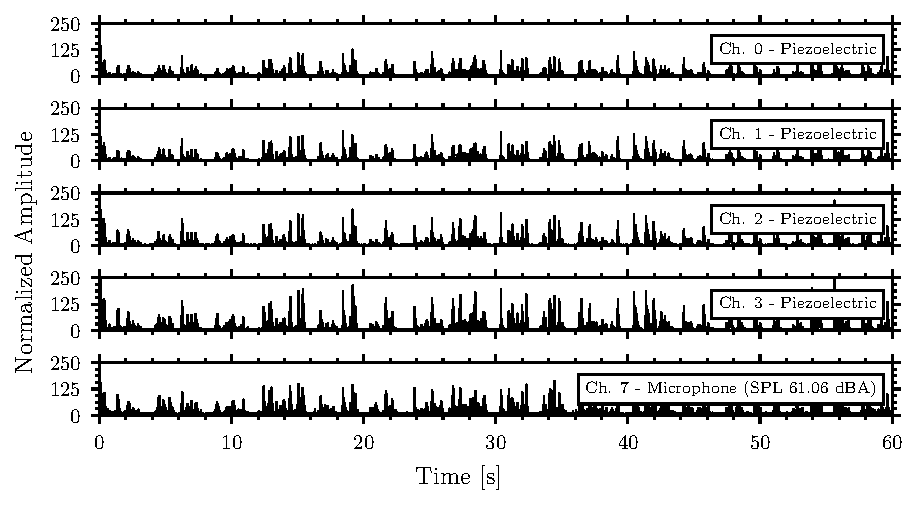
\includegraphics[width=\textwidth]{figures/external_noise/waveform_41.pdf}
% 	\caption{Waveform display of \SI{60}{\deci\bel A} external noise}
% 	\label{fig:waveform_41}
% \end{figure}

% \newpage 

% The NSPA and NSEL measurements of records when external noise present are shown in Table \ref{tab:nspa_external_noise}:

% \begin{table}[htbp!]
% 	\centering
% 	\caption{NSPA and NSEL of the maximum internal piezoelectric disc and externally mounted microphone, channel seven, during various levels of background noise \label{tab:nspa_external_noise}}
% 	\begin{tabular}{rrrrr}
% 		\toprule
% 		\multirow{2}{*}{\textbf{Noise Level [\si{\deci\bel A}]} } & \multicolumn{2}{c}{\textbf{Internal}} & \multicolumn{2}{c}{\textbf{External (Ch. 7)}}                                 \\
% 		                                                          & \textbf{NSPA}                         & \textbf{NSEL}                                 & \textbf{NSPA} & \textbf{NSEL} \\
% 		\midrule
% 		60                                                        & 44.06                                 & 29.97                                         & 40.55         & 27.45         \\
% 		70                                                        & 50.86                                 & 33.99                                         & 46.93         & 31.60         \\
% 		80                                                        & 60.57                                 & 44.00                                         & 56.46         & 40.80         \\
% 		90                                                        & 61.48                                 & 47.46                                         & 59.63         & 45.67         \\
% 		\bottomrule
% 	\end{tabular}
% \end{table}

% Not only do the internal piezoelectric discs exhibit a higher NSPA and NSEL compared to the external microphone, but the magnitude of the metric surpasses the insect measurements shown in Table \ref{tab:nspa_nsel_comparison}. This signifies that the NSPA and NSEL measurements, when extracted within the \SIrange{500}{6000}{\hertz} band, are highly susceptible by the influence of external noise.

% \newpage
% The NSPA algorithm was parametrized in order to find the lower and upper frequency limits that would enable the optimal detection of insect signals while minimizing the impact of external noise. This was performed by minimizing the difference between the NSPA calculated for a record containing an insect and no external noise with a record with no insect and external noise. Figure \ref{fig:frequency_finder} shows the process of minimizing the NSPA difference, first to find the lower frequency limit and then the upper frequency limit. The lower and upper frequency bounds were found to be \SI{1625}{\hertz} and \SI{5400}{\hertz}, respectively.

% \begin{figure}[!htbp]
% 	\centering
% 	\begin{subfigure}{\textwidth}
% 		\centering
% 		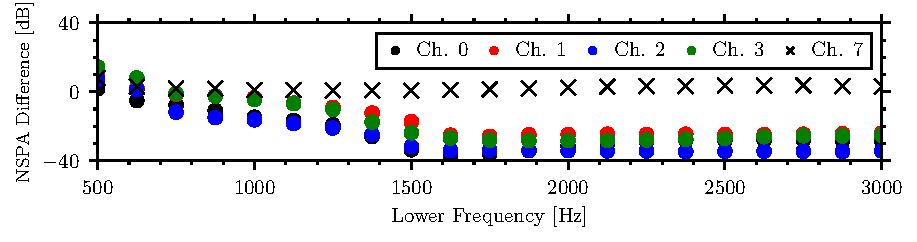
\includegraphics[width=\textwidth]{figures/external_noise/lower_frequency_nspa_difference.pdf}
% 		\caption{Lower Frequency Limit}
% 		\label{fig:lower_freq_limit}
% 	\end{subfigure}

% 	\begin{subfigure}{\textwidth}
% 		\centering
% 		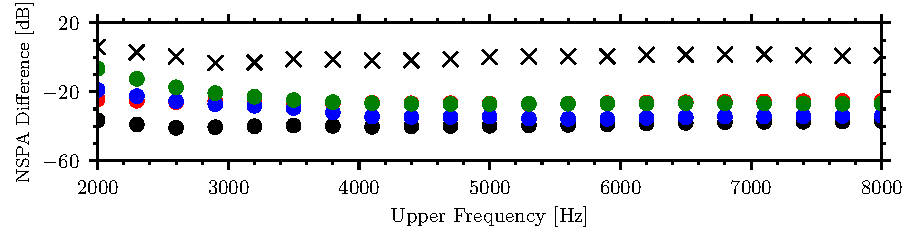
\includegraphics[width=\textwidth]{figures/external_noise/upper_frequency_nspa_difference.pdf}
% 		\caption{Upper Frequency Limit}
% 		\label{fig:upper_freq_limit}
% 	\end{subfigure}

% 	\caption{Finding frequency limits to minimize NSPA difference }%
% 	\label{fig:frequency_finder}
% \end{figure}

% Table \ref{tab:optimal_frequency} shows the NSPA values when using the frequency range \SIrange{1625}{5400}{\hertz} for the \textit{T. confusum} in flour and external noise with no insect. Even at \SI{90}{\deci\bel A} external noise, the NSPA of the internal piezoelectric channels do not exceed the levels experienced when an insect is present.

% \begin{table}[htbp!]
% 	\centering
% 	\caption{NSPA of internal piezoelectric disc and externally mounted microphone, channel seven, during \textit{T. confusum} in flour external noise with no insect and using the optimal frequency range \SIrange{1625}{5400}{\hertz} \label{tab:optimal_frequency}}
% 	\begin{tabular}{lrrrrrr}
% 		\toprule
% 		\textbf{Subject}     & \textbf{Ch. 0 [\si{\deci\bel}]} & \textbf{Ch. 1 [\si{\deci\bel}]} & \textbf{Ch. 2 [\si{\deci\bel}]} & \textbf{Ch. 3 [\si{\deci\bel}]} & \textbf{Ch. 7 [\si{\deci\bel}]} & \textbf{SPL [dBA]} \\
% 		\midrule
% 		\textit{T. confusum} & 48.57                           & 37.75                           & 44.70                           & 42.53                           & 41.45                           & 32.46              \\
% 		Noise (No insect)    & 9.15                            & 10.71                           & 9.12                            & 15.54                           & 41.92                           & 68.46              \\
% 		Noise (No insect)    & 15.36                           & 17.30                           & 19.83                           & 24.04                           & 51.08                           & 80.95              \\
% 		Noise (No insect)    & 21.24                           & 23.65                           & 25.41                           & 30.42                           & 60.11                           & 89.88              \\
% 		\bottomrule
% 	\end{tabular}
% \end{table}